\documentclass[11pt]{article}

\usepackage[margin=1in]{geometry}
\usepackage{amsmath}
\usepackage{amssymb}
\usepackage{booktabs}
\usepackage{graphicx}
\usepackage{hyperref}
\usepackage{listings}
\usepackage{tikz}
\usepackage{xcolor}
\usetikzlibrary{arrows.meta,positioning}

\hypersetup{
  colorlinks=true,
  linkcolor=blue!55!black,
  citecolor=blue!55!black,
  urlcolor=blue!55!black
}

\lstset{
  basicstyle=\ttfamily\small,
  breaklines=true,
  frame=single,
  columns=fullflexible
}

\newcommand{\WiscAuthors}{Juha Vierinen \and Bj{\"o}rn Gustavsson}

\title{WISC: A Browser-Based Widefield Star Calibrator}
\author{\WiscAuthors}
\date{Draft for WISC v0.2.18}

\begin{document}
\maketitle

\begin{abstract}
We describe a browser-based calibration tool for fitting wide-field camera
models to images of the night sky. The application combines manual star
pairing, automatic bright-star detection, blind asterism matching, robust
nonlinear optimization, residual inspection, and code export in a self-contained
HTML and JavaScript interface. The current implementation is designed for
wide-field and all-sky cameras with fields of view above roughly 30 degrees and
stars brighter than visual magnitude 7. It uses simple but sufficiently
malleable parametric lens models that are known to work on a wide range of
wide-field cameras, including fisheye lenses used in auroral research, and it
also supports a Brown-Conrady model for ordinary phone cameras. The tool
emphasizes practical calibration under imperfect observing conditions,
including aurora, buildings, image noise, nonlinear lens effects, and spurious
star detections. Recent development has focused on making full-horizon fisheye
images easier to initialize automatically by detecting the circular horizon
annulus, inferring approximate camera center and scale, and using those
quantities to seed the fisheye model before star association.
\end{abstract}

\section{Introduction}

Wide-field optical calibration is needed when image pixels must be mapped to
sky directions. Examples include all-sky auroral imaging, meteor cameras,
planetarium-style camera alignment, and phone-camera photographs of bright
stars. Traditional calibration workflows often combine several separate tools:
image viewers, star catalogs, custom fitting scripts, and hand-written export
code. WISC packages these steps into one application.

The application is intentionally local and transparent. Images are loaded in the
browser. The bright-star catalog is embedded in JavaScript. The lens model,
projection, star detection, asterism matching, fitting, residual analysis, and
export routines are all implemented client-side. When served by the local
development server, the application can also save calibrated test cases for
regression testing.

\section{User Workflow}

The workflow is centered on matching image detections to catalog stars. The user
loads an image, verifies the UTC timestamp and observer location, selects a
lens model, and roughly aligns the sky projection. The application supports
manual pairing through a keyboard-modified click workflow. Holding \texttt{S}
and clicking near an image star opens a local density estimate; the centroid is
refined at subpixel resolution and can then be paired with a catalog star.
If the same modified click is performed over an existing pair, the pair can be
removed without entering a separate editing mode.

The ``I'm feeling lucky'' path automates the same idea. It detects bright image
features, attempts a blind spherical asterism match, seeds the selected optical
model, expands the number of candidate matches, fits the lens parameters, and
rejects obvious outliers. The user can paint bad star-finder regions with
\texttt{M}+click. These marked regions remove yellow automatic detections from
future automatic matching and are saved with submitted test-case metadata.

For all-sky fisheye images, the application also tries to recognize the dark
outside-of-horizon annulus when the image is loaded. If a circular horizon is
detected, the browser switches to the fisheye model and initializes the optical
center, focal scale, and radial parameter from the measured horizon circle.
This is particularly useful for ALIS-style and similar all-sky images where the
image contains a nearly complete horizon ring.

\section{Metadata Inference}

Correct time and observer location are critical because the catalog sky is
local. WISC therefore tries several metadata sources before requiring manual
entry. The preferred source is EXIF metadata, including GPS position, altitude,
image direction, and timestamp when these fields are present. When EXIF data
are missing or incomplete, the browser falls back to filename conventions for
known image sources. Supported patterns include allsky7-style names with
underscore-separated timestamps and camera identifiers, IRF/ALIS-style names
such as \texttt{2026-01-23T20.05.00.000KRN.jpeg}, and compact station names
such as \texttt{20260112173523\_RAM.jpg}. In the latter example, \texttt{RAM}
is interpreted as Ramfjordmoen, with site coordinates \(69.5860^\circ\) N,
\(19.2247^\circ\) E and altitude \(0\ \mathrm{m}\).

\begin{table}[h]
\centering
\begin{tabular}{lll}
\toprule
Filename form & Parsed fields & Example station metadata \\
\midrule
\texttt{YYYY\_MM\_DD\_hh\_mm\_ss\_ID} & UTC time, allsky7 ID & coarsened allsky7 site \\
\texttt{YYYY-MM-DDThh.mm.ss.sssKRN} & UTC time, ALIS code & Kiruna IRF \\
\texttt{YYYYMMDDhhmmss\_RAM} & UTC time, compact code & Ramfjordmoen \\
\bottomrule
\end{tabular}
\caption{Filename metadata conventions currently understood by WISC. Manual
metadata entry remains available and overrides inferred values.}
\label{tab:metadata-inference}
\end{table}

\section{Coordinate Systems}

The application uses true zero-based image pixel coordinates in the browser. A
catalog star is first converted from right ascension and declination to local
azimuth and zenith angle using the image timestamp and observer position. Let
\(\alpha_\star\) be right ascension, \(\delta_\star\) declination, \(\phi\) the
observer latitude, and \(H\) the local hour angle. The altitude is
\begin{equation}
  h = \sin^{-1}\left(\cos H \cos\delta_\star \cos\phi
      + \sin\delta_\star \sin\phi\right),
\end{equation}
and the zenith angle is
\begin{equation}
  z = \frac{\pi}{2} - h.
\end{equation}
The local sky unit vector used by the browser projection model is
\begin{equation}
  \mathbf{e} =
  \begin{bmatrix}
    \sin z \sin A \\
    \sin z \cos A \\
    \cos z
  \end{bmatrix},
\end{equation}
where \(A\) is azimuth.

\section{Camera Rotation and Projection}

The browser implementation uses a three-angle camera rotation convention
compatible with the historical calibration tools. The rotation matrix is
\begin{equation}
  R = R_y(\alpha) R_x(\beta) R_z(\gamma).
\end{equation}
The local sky vector is transformed into camera coordinates by
\begin{equation}
  \mathbf{s} = \mathbf{e} R,
  \qquad
  \mathbf{s} = (s_1, s_2, s_3).
\end{equation}
Here \(\mathbf{s}\) is no longer an east--north--up vector. It is the same
unit ray expressed in the camera frame. The first two components,
\(s_1\) and \(s_2\), are the horizontal and vertical coordinates in the
camera image plane, while \(s_3\) is the coordinate along the optical axis
or boresight. Thus a point near the center of the image has small
\(s_1\) and \(s_2\) compared with \(s_3\), and the ratios \(s_1/s_3\) and
\(s_2/s_3\) are the usual rectilinear normalized image-plane coordinates.

\begin{figure}[h]
\centering
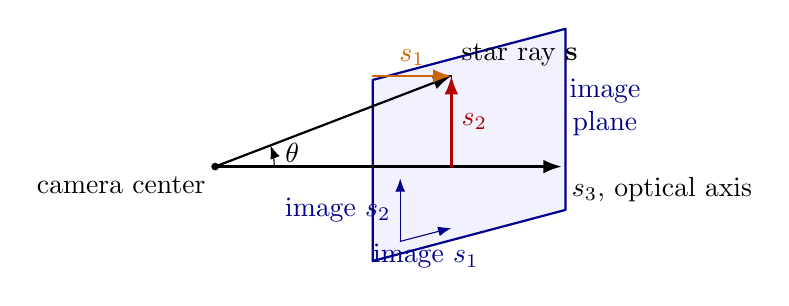
\begin{tikzpicture}[scale=1.0, >=Latex, line cap=round, line join=round]
  \coordinate (O) at (0,0);
  \coordinate (P) at (3.0,1.15);
  \coordinate (S1) at (3.0,0);
  \coordinate (S2) at (3.0,1.15);
  \coordinate (S3) at (4.2,-1.0);

  \fill[blue!5] (2.0,-1.2) -- (4.45,-0.55) -- (4.45,1.75) -- (2.0,1.1) -- cycle;
  \draw[blue!55!black, thick] (2.0,-1.2) -- (4.45,-0.55) -- (4.45,1.75) -- (2.0,1.1) -- cycle;
  \node[blue!55!black, align=center] at (4.95,0.75) {image\\plane};

  \draw[->, thick] (O) -- (4.4,0) node[below right] {\(s_3\), optical axis};
  \draw[->, thick] (O) -- (P) node[above right] {star ray \(\mathbf{s}\)};
  \draw[dashed] (P) -- (3.0,0);
  \draw[dashed] (P) -- (2.0,1.15);
  \draw[->, thick, red!70!black] (3.0,0) -- (P) node[midway,right] {\(s_2\)};
  \draw[->, thick, orange!80!black] (2.0,1.15) -- (P) node[midway,above] {\(s_1\)};

  \draw[->, blue!55!black] (2.35,-0.95) -- (3.0,-0.78) node[midway,below] {image \(s_1\)};
  \draw[->, blue!55!black] (2.35,-0.95) -- (2.35,-0.15) node[midway,left] {image \(s_2\)};

  \draw[->] (0.75,0) arc[start angle=0,end angle=21,radius=0.75];
  \node at (0.98,0.18) {\(\theta\)};
  \fill (O) circle (1.4pt) node[below left] {camera center};
\end{tikzpicture}
\caption{Meaning of the camera-frame components. After rotation from local
east--north--up coordinates, the same unit star ray is represented as
\(\mathbf{s}=(s_1,s_2,s_3)\). The \(s_3\) axis is the optical axis. The
\(s_1\) and \(s_2\) components locate where the ray pierces the camera image
plane, and their ratios to \(s_3\) give the rectilinear normalized image
coordinates.}
\label{fig:camera-frame-components}
\end{figure}

The radial angle from the optical axis is
\begin{equation}
  \theta = \tan^{-1}\left(\frac{\sqrt{s_1^2+s_2^2}}{s_3}\right).
\end{equation}

For the sine-like fisheye model, exposed in the interface as
\texttt{optmod 2}, the radial mapping is
\begin{equation}
  r = \sin(a_r \theta),
\end{equation}
and the normalized pixel coordinates are
\begin{align}
  u &= f_1 \frac{s_1}{\sqrt{s_1^2+s_2^2}} r + \frac{1}{2} + d_u, \\
  v &= f_2 \frac{s_2}{\sqrt{s_1^2+s_2^2}} r + \frac{1}{2} + d_v.
\end{align}
The browser pixel coordinates are then
\begin{equation}
  x = u W - 1, \qquad y = v H - 1,
\end{equation}
where \(W\) and \(H\) are image width and height. The \(-1\) term converts from
the historical MATLAB one-based convention to browser zero-based coordinates.

\section{Supported Lens Models}

The current browser supports a family of simple but sufficiently malleable
parametric lens models, exposed as \texttt{optmod 1}, \texttt{2}, \texttt{3},
\texttt{4}, \texttt{5}, and \texttt{12}. These models are not intended to be
complete physical descriptions of a lens. They are compact radial projection
laws that have been found to fit a wide range of wide-field cameras in
practice, including fisheye lenses used in auroral research. They share the
parameter vector
\begin{equation}
  \mathbf{p} = [f_1, f_2, \alpha, \beta, \gamma, d_u, d_v, a_r].
\end{equation}
The browser also supports a Brown-Conrady model, called \texttt{optmod 20} in
the interface, with radial and tangential coefficients:
\begin{equation}
  \mathbf{p}_{BC} =
  [f_1, f_2, \alpha, \beta, \gamma, d_u, d_v,
   k_1, k_2, k_3, p_1, p_2].
\end{equation}

\begin{table}[h]
\centering
\begin{tabular}{lll}
\toprule
Model & Use case & Notes \\
\midrule
Optmod 2 & all-sky and fisheye cameras & \(\sin(a_r\theta)\) radial law \\
Optmod 12 & flexible wide-field lenses & tangent/sine branch by sign \\
Brown-Conrady & phone and ordinary lenses & radial plus tangential distortion \\
\bottomrule
\end{tabular}
\caption{Common model choices in the browser calibrator.}
\end{table}

\section{Fisheye Horizon Initialization}

For full-horizon fisheye images, WISC includes a fast horizon-annulus detector.
The detector uses the fact that many all-sky images contain a bright circular
field surrounded by nearly black pixels. Sparse text labels, cardinal-direction
annotations, and timestamps can be present, so the detector does not simply use
a mean edge profile. It first scans horizontal and vertical lines to find
threshold crossings between the illuminated field and the black outside region.
The resulting edge points are fitted with a robust circle fit. Outlying edge
points are iteratively trimmed, which makes the estimate insensitive to
annotation text and small non-circular artifacts.

The fitted circle provides an initial optical center and horizon radius. The
center search is allowed to move by up to roughly \(10\%\) of the image size
from the image midpoint. This matters because real all-sky camera images are
not always perfectly centered in the stored pixel array. After the robust
circle fit, a radial peak-density profile is evaluated around the fitted center
to measure the horizon edge. The relevant score is the drop in the modal
intensity density between samples just inside and just outside the horizon:
\begin{equation}
  S(r) =
  \mathrm{mode}\{I(\rho < r)\} -
  \mathrm{mode}\{I(\rho > r)\},
\end{equation}
where the modes are estimated from small radial windows around the candidate
edge. The correct center makes the horizon circle coherent, and therefore
maximizes this radial density drop more sharply than an offset center.

The detected radius is converted to an initial \texttt{optmod 2} focal scale
using the sine fisheye model. If the fitted horizon radius is \(R_h\), image
width is \(W\), and the initial radial parameter is \(a_r\), the initial
horizontal focal parameter is
\begin{equation}
  f_1 \approx \frac{R_h/W}{\sin(a_r\pi/2)}.
\end{equation}
The vertical focal parameter follows from the image aspect ratio. On the KRN
fisheye validation case, the horizon detector runs in about one second on a
standard development machine and places the center within a few tenths of a
pixel of the manually saved horizon center. The validation report records this
runtime explicitly so that later changes do not silently make image loading
slow.

\section{Star Detection}

Automatic detection starts from a grayscale representation of the input image.
The detector estimates local and global brightness structure, thresholds
candidate peaks, suppresses nearby duplicates, and rejects obviously elongated
or crowded detections. Detected stars are ranked by contrast and flux-like
scores. Painted bad regions are applied as exclusion masks before automatic
pairing, allowing the user to remove spurious detections from buildings,
aurora, hot pixels, or image artifacts.
This design follows the practical lessons of Source Extractor
\cite{bertin1996sextractor} and SEP \cite{barbary2016sep}: estimate a
spatially variable background and noise field, use a compact PSF-like matched
filter to favor point sources, and treat segmentation/deblending ideas as a way
to prevent extended structures from masquerading as stars. The browser
implementation does not expose these as user tuning parameters. Instead, it
uses automatic local background estimates and matched-filter peak scoring
inside the detector, with mesh background/RMS estimation retained as an
oracle-tested diagnostic option rather than a mandatory GUI setting. Detector
changes are validated offline with oracle tests that compare detections against
catalog stars projected through known lens models.

Manual picking uses a different path. The user clicks near a star and the tool
extracts a local image patch. A smoothed density estimate is computed on an
interpolated grid, and the local peak is used as the subpixel image coordinate.
This gives the user a controlled way to create high-confidence calibration
pairs even when automatic detection is confused.

\section{Asterism Matching}

The browser contains two matching strategies. The projected matcher uses the
current lens model to project catalog stars into the image and then performs
nearest-neighbor matching with robust filtering. This works well after the
model is already roughly aligned. The blind matcher is more important for the
``I'm feeling lucky'' workflow because it must establish an initial sky
orientation before a useful lens fit exists.

\subsection{Current Blind Matcher}

The current blind matcher is a local, browser-sized version of an astrometric
index. It does not use a precomputed all-sky quad index. Instead, for each
image and observing time it builds a temporary index from stars that are above
the local horizon and bright enough for the current search stage.
In the code this is the blind-detection stage of the lucky solver: it tries to
turn a list of anonymous image peaks into named catalog-star associations
without first knowing the camera pointing.

The main input sets are:
\begin{enumerate}
  \item image detections \(\mathcal{D}=\{d_i\}\), sorted by star-detector
        score;
  \item visible catalog stars \(\mathcal{C}=\{c_j\}\), sorted by visual
        magnitude;
  \item a small grid of pre-flattening lens guesses, including candidate
        focal scales, radial parameters, signs, and approximate projection
        families.
\end{enumerate}
The browser display can use Tycho--2 for deeper star rendering, but the current
lucky fitting path deliberately uses the Yale bright-star catalog for its
automatic bootstrap. This keeps the matching problem smaller and preserves the
well-tested behavior of older successful cases. Deeper Tycho--2 stars are still
valuable for display, manual inspection, and future experiments, but simply
adding many fainter catalog stars is not a cure for bad bootstrap detections.

Astrometry.net uses a related but stronger idea based on four-star
asterisms, usually called quads. In a quad, two stars are labeled \(A\) and
\(B\) and used as the backbone that fixes translation, scale, and rotation.
The remaining stars, \(C\) and \(D\), are then described by their normalized
coordinates in the coordinate system defined by the \(A\)--\(B\) backbone.
If an image quad and a catalog quad have nearby normalized \(C,D\)
coordinates, the two quads are considered a matching quad. This is only a
hypothesis: astrometry.net then verifies the implied sky solution by checking
whether many additional catalog stars land on image detections.

\begin{figure}[h]
\centering
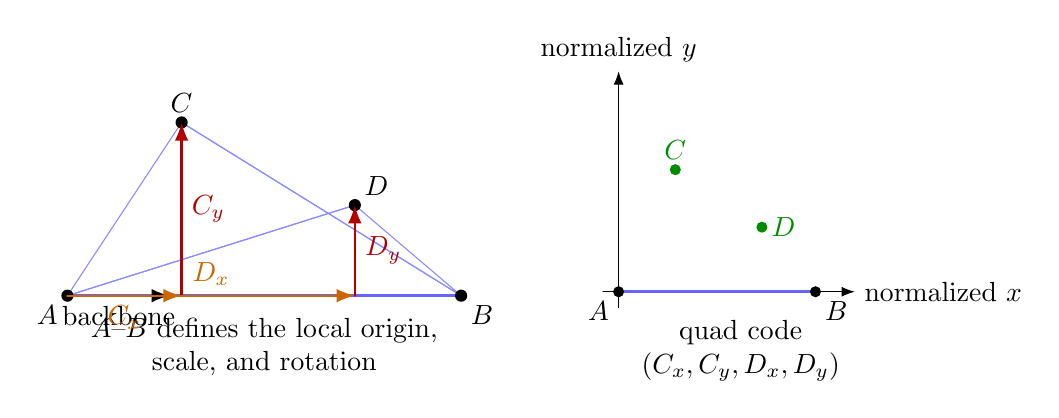
\begin{tikzpicture}[scale=1.0, >=Latex, line cap=round, line join=round]
  \coordinate (A) at (0,0);
  \coordinate (B) at (5.0,0);
  \coordinate (C) at (1.45,2.2);
  \coordinate (D) at (3.65,1.15);

  \draw[very thick, blue!60] (A) -- (B);
  \draw[blue!45] (A) -- (C) -- (B) -- (D) -- cycle;
  \draw[blue!45] (A) -- (D);
  \draw[blue!45] (B) -- (C);

  \fill[black] (A) circle (2.2pt) node[below left] {\(A\)};
  \fill[black] (B) circle (2.2pt) node[below right] {\(B\)};
  \fill[black] (C) circle (2.2pt) node[above] {\(C\)};
  \fill[black] (D) circle (2.2pt) node[above right] {\(D\)};

  \draw[->, thick] (A) -- (1.3,0) node[midway,below] {backbone};
  \node[align=center] at (2.5,-0.65)
      {\(A\)--\(B\) defines the local origin,\\scale, and rotation};

  \draw[dashed] (C) -- (1.45,0);
  \draw[dashed] (D) -- (3.65,0);
  \draw[->, red!70!black, thick] (1.45,0) -- (C)
      node[midway,right] {\(C_y\)};
  \draw[->, orange!80!black, thick] (A) -- (1.45,0)
      node[midway,below] {\(C_x\)};
  \draw[->, red!70!black, thick] (3.65,0) -- (D)
      node[midway,right] {\(D_y\)};
  \draw[->, orange!80!black, thick] (A) -- (3.65,0)
      node[midway,above] {\(D_x\)};

  \begin{scope}[xshift=7.0cm, yshift=0.05cm]
    \draw[->] (-0.2,0) -- (3.0,0) node[right] {normalized \(x\)};
    \draw[->] (0,-0.2) -- (0,2.8) node[above] {normalized \(y\)};
    \draw[very thick, blue!60] (0,0) -- (2.5,0);
    \fill[black] (0,0) circle (2pt) node[below left] {\(A\)};
    \fill[black] (2.5,0) circle (2pt) node[below right] {\(B\)};
    \fill[green!55!black] (0.72,1.55) circle (2pt) node[above] {\(C\)};
    \fill[green!55!black] (1.82,0.82) circle (2pt) node[right] {\(D\)};
    \node[align=center] at (1.55,-0.75)
        {quad code\\\((C_x,C_y,D_x,D_y)\)};
  \end{scope}
\end{tikzpicture}
\caption{Astrometry.net-style quad geometry. Stars \(A\) and \(B\) form a
backbone. After translating, rotating, and scaling by this backbone, the
positions of \(C\) and \(D\) form a scale-free, rotation-free quad code. A
matching quad is a catalog quad whose code is close to the image quad code.
The quad match is only a proposal; the proposed sky solution is accepted only
after additional stars support it.}
\label{fig:quad-signature}
\end{figure}

For a candidate pre-flattening model, every selected image detection is mapped
from pixel coordinates into an approximate unit vector
\(\tilde{\mathbf{v}}_i\). The mapping is intentionally rough: its purpose is
not to calibrate the lens, but to make triangle side lengths in image space
comparable with angular side lengths in the sky. Catalog stars are converted to
local sky unit vectors \(\mathbf{u}_j\) from the timestamp and observer
location.

\begin{figure}[h]
\centering
\resizebox{\linewidth}{!}{%
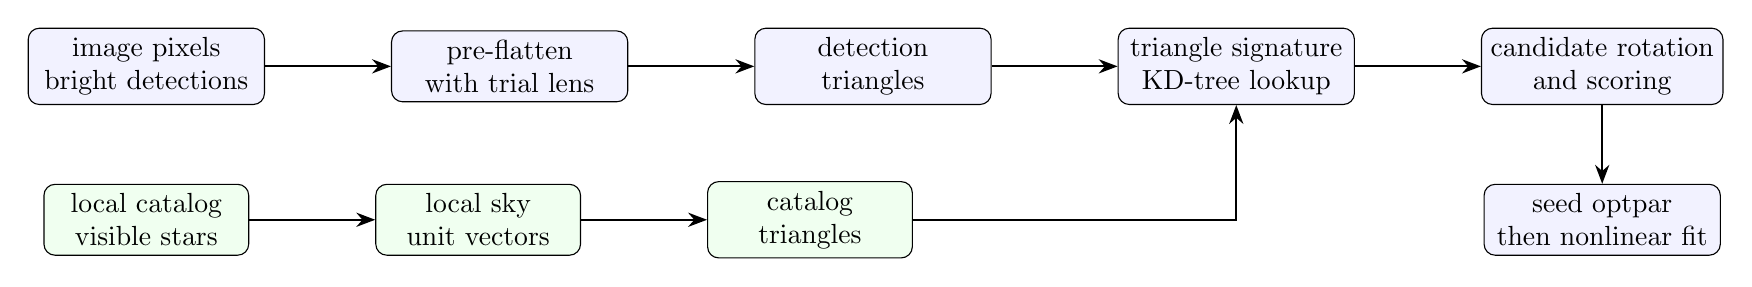
\begin{tikzpicture}[
    node distance=1.2cm,
    box/.style={draw, rounded corners, align=center, minimum width=3.0cm,
                minimum height=0.9cm, fill=blue!5},
    smallbox/.style={draw, rounded corners, align=center, minimum width=2.6cm,
                minimum height=0.75cm, fill=green!6},
    arrow/.style={-{Stealth[length=2.4mm]}, thick}
]
  \node[box] (img) {image pixels\\bright detections};
  \node[box, right=1.6cm of img] (flat) {pre-flatten\\with trial lens};
  \node[box, right=1.6cm of flat] (triimg) {detection\\triangles};
  \node[smallbox, below=1.0cm of img] (cat) {local catalog\\visible stars};
  \node[smallbox, right=1.6cm of cat] (sky) {local sky\\unit vectors};
  \node[smallbox, right=1.6cm of sky] (tric) {catalog\\triangles};
  \node[box, right=1.6cm of triimg] (kd) {triangle signature\\KD-tree lookup};
  \node[box, right=1.6cm of kd] (rot) {candidate rotation\\and scoring};
  \node[box, below=1.0cm of rot] (seed) {seed optpar\\then nonlinear fit};

  \draw[arrow] (img) -- (flat);
  \draw[arrow] (flat) -- (triimg);
  \draw[arrow] (cat) -- (sky);
  \draw[arrow] (sky) -- (tric);
  \draw[arrow] (triimg) -- (kd);
  \draw[arrow] (tric) -| (kd);
  \draw[arrow] (kd) -- (rot);
  \draw[arrow] (rot) -- (seed);
\end{tikzpicture}
}
\caption{Current browser blind-matching pipeline. The catalog index is built
on demand for the local sky at the image time. The detection side is rebuilt
for several approximate lens pre-flattening hypotheses.}
\label{fig:asterism-pipeline}
\end{figure}

\subsection{Blind Detection As Implemented}

The current blind-detection loop can be summarized as follows. First, the image
star detector produces a ranked list of compact local maxima. The ranking is
not simply brightness. It combines peak contrast, aperture flux, compactness,
core concentration, peak dominance, elongation, saturation, local crowding, and
matched-filter signal-to-noise. This ranking is useful for suppressing aurora,
buildings, clouds, hot pixels, and compression artifacts, but it can still be
fooled by sharp non-stellar features or by real but geometrically unhelpful
faint stars.

Second, the lucky solver selects only the first \(N\) detections for a stage.
For Brown--Conrady phone-image bootstraps, typical stages use \(N=80\), then
\(N=160\), and then a deeper stage with more detections if no seed has been
accepted. For the allsky7-like optmod-2 path, the early \(N\) values are kept
smaller and the pre-flattening grid is more constrained, because that recipe is
known to work for full-sky fisheye images.

Third, the selected detections are pre-flattened by each trial lens guess. In
the Brown--Conrady blind stage this pre-flattening is intentionally simple:
pixel coordinates are treated as approximately pinhole rays, with the focal
scale searched over a small grid and with the \(f_1/f_2\) ratio initialized
from the image aspect ratio. The Brown--Conrady radial and tangential
coefficients are not used to generate the blind asterisms; they are fitted only
after star pairings have been established. For optmod 2, the trial grid also
includes the radial parameter \(a_r\).

Fourth, the code builds image triangles and catalog triangles, compares their
\((a/c,b/c)\) signatures, and scores the rotation hypotheses implied by nearby
signature pairs. The score is based on how many catalog stars are explained by
the same rotation, the angular residuals, ambiguity checks, and conflicts. A
candidate that explains only its seed triangle is not trusted. It must extend
to other stars, and later projected stages are guarded by pixel-space RMS so
that bad additions can be rejected.

The important practical consequence is that the blind matcher is only as good
as the early detection list. If the first detections contain enough real stars
with approximately correct centroids, the triangle matcher is quite robust. If
the same list is dominated by false positives, locally repeated texture, or
stars that are a poor geometric subset, the matcher can find a self-consistent
but wrong sky orientation. In that failure mode, increasing the catalog depth
may make the ambiguity worse rather than better.

\subsection{Triangle Signature}

For each set of candidate points, the matcher builds triangular asterisms. For
a triangle with side lengths \(a\le b\le c\), the current signature is a
two-dimensional, scale-free descriptor
\begin{equation}
  \mathbf{q} =
  \begin{bmatrix}
    a/c\\
    b/c
  \end{bmatrix}.
\end{equation}
Degenerate triangles are rejected before indexing. The three vertices must be
distinct detections or catalog stars, so the same star candidate cannot appear
twice in one triangle. For image-detection triangles, the shortest pixel side
must also be at least
\begin{equation}
  N_{\mathrm{MIN\_ANGLE\_PIX}} = 50 \ \mathrm{px}.
\end{equation}
Conversely, the longest pixel side must not exceed one quarter of the image
width,
\begin{equation}
  c \le \frac{W}{4}.
\end{equation}
This prevents very large triangles from dominating the search. Such triangles
are a poor choice for wide lenses because small radial-model errors near the
edge of the field produce large changes in their side ratios. After these
pixel-scale checks, the matcher still requires a minimum shortest-to-longest
side ratio and a minimum area relative to \(c^2\). These tests remove tiny,
duplicate, over-wide, and nearly collinear triples, which are poor rotation
constraints and are common in noisy detections.

Catalog triangle signatures are inserted into a two-dimensional KD-tree. For
each image-detection triangle, the matcher searches the KD-tree for nearby
catalog signatures. A nearby signature does not prove an identification; it
only proposes a candidate correspondence between three image detections and
three catalog stars. Each proposed correspondence gives a rotation hypothesis.
For the spherical matcher, the rotation is estimated from two vector pairs and
the third vertex is used as a consistency check. The rotation is then scored
against all available stars, not just the three that generated the hypothesis.

\begin{figure}[h]
\centering
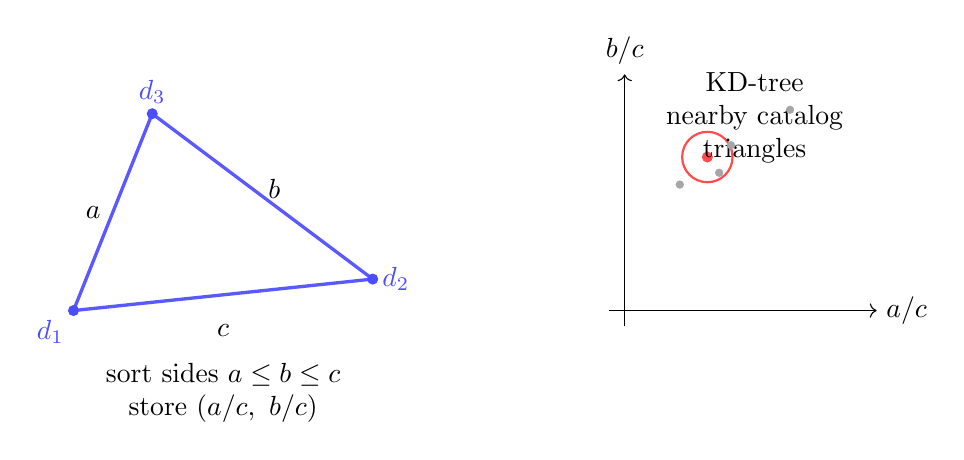
\begin{tikzpicture}[scale=1.0]
  \coordinate (a) at (0,0);
  \coordinate (b) at (3.8,0.4);
  \coordinate (c) at (1.0,2.5);
  \draw[very thick, blue!65] (a) -- (b) -- (c) -- cycle;
  \fill[blue!70] (a) circle (2pt) node[below left] {\(d_1\)};
  \fill[blue!70] (b) circle (2pt) node[right] {\(d_2\)};
  \fill[blue!70] (c) circle (2pt) node[above] {\(d_3\)};
  \node at (1.9,-0.25) {\(c\)};
  \node at (2.55,1.55) {\(b\)};
  \node at (0.25,1.25) {\(a\)};
  \node[align=center] at (1.9,-1.05)
      {sort sides \(a\le b\le c\)\\store \((a/c,\ b/c)\)};

  \begin{scope}[xshift=7.0cm]
    \draw[->] (-0.2,0) -- (3.2,0) node[right] {\(a/c\)};
    \draw[->] (0,-0.2) -- (0,3.0) node[above] {\(b/c\)};
    \fill[red!70] (1.05,1.95) circle (2pt);
    \draw[red!70, thick] (1.05,1.95) circle (0.32);
    \node[align=center] at (1.65,2.45) {KD-tree\\nearby catalog\\triangles};
    \fill[gray!70] (0.7,1.6) circle (1.5pt);
    \fill[gray!70] (1.2,1.75) circle (1.5pt);
    \fill[gray!70] (1.35,2.1) circle (1.5pt);
    \fill[gray!70] (2.1,2.55) circle (1.5pt);
  \end{scope}
\end{tikzpicture}
\caption{Triangle signatures remove overall scale by using side ratios. A
candidate image triangle queries a KD-tree of catalog triangle signatures; each
near neighbor proposes a possible three-star correspondence.}
\label{fig:triangle-signature}
\end{figure}

\subsection{Rejected Gradient Diagnostic}

An earlier prototype also estimated local direction-cosine gradients for each
candidate triangle. The idea was to use finite differences of the east and
north sky-vector components with respect to image \(x\) and \(y\). In practice
these measurements were too noisy for fisheye and other very wide field
images, and they did not improve candidate selection beyond the triangle
signature and support-triangle checks. The current browser implementation does
not compute or filter on these gradients during asterism search.

\subsection{Candidate Scoring and Seeding}

A triangle correspondence is accepted only if it explains additional stars.
After a candidate rotation \(R_k\) is generated, every pre-flattened detection
vector is rotated into the catalog frame and matched to nearby catalog vectors.
The candidate score increases with the number and brightness of consistent
matches and decreases with angular residuals, ambiguous alternatives, and
conflicts. The chosen candidate returns:
\begin{itemize}
  \item matched image detections and catalog stars;
  \item the approximate camera rotation;
  \item the pre-flattening parameters that generated the best detection
        vectors;
  \item diagnostic counts such as scored rotations and triangle counts.
\end{itemize}
The browser converts the recovered rotation into the selected camera-angle
parameterization and seeds the selected lens model. Subsequent Levenberg-Marquardt and
Nelder-Mead sweeps operate in pixel space and no longer rely on the triangle
signature approximation.

\subsection{Lucky Search Stages}

The ``I'm feeling lucky'' workflow is a staged bootstrap and refinement
procedure. It is designed to avoid committing to weak, ambiguous detections
until there is some evidence that the image and catalog are already on the
same geometric track. The main steps are:
\begin{enumerate}
  \item \textbf{Detect compact bright peaks.} The detector ranks candidate
        peaks by contrast, flux, compactness, central concentration, peak
        dominance, low outer-aperture flux, elongation, saturation, and local
        crowding. Bad star-finder regions painted by the user are masked.
  \item \textbf{Blind spherical bootstrap.} Candidate image detections are
        pre-flattened with a small grid of lens hypotheses and converted to
        unit vectors. Triangular asterisms from the image are matched against
        local catalog triangles. Some blind-search modes can request regional
        detection coverage so that one cluttered part of the frame does not
        dominate the selected detections, but the current Brown--Conrady lucky
        recipe primarily relies on whole-image detections and global scoring.
  \item \textbf{Support-triangle verification.} A seed asterism is not accepted
        by itself. The candidate rotation must extend to neighboring stars:
        each seed star is tested in additional triangles with nearby provisional
        matches. These support triangles use the same minimum side length,
        maximum side length, and minimum height limits as the main asterisms.
        Accepted support triangles can be drawn in the GUI as diagnostic
        asterisms while the search is running.
  \item \textbf{Stop on an empty first stage.} If the first blind asterism
        stage finds no matched stars, the lucky workflow stops. It does not
        proceed to fainter stars, because the later stages would otherwise have
        a high chance of following noise or non-star structure.
  \item \textbf{Seed the lens model and fit bright pairs.} A successful blind
        match gives an approximate camera rotation and pre-flattening lens
        parameters. These seed the selected lens model. The browser then fits
        the brightest automatic pairs first with robust Nelder-Mead and
        Levenberg-Marquardt sweeps.
  \item \textbf{Add weaker stars cautiously.} Once a model exists, later stages
        use projected catalog positions to add fainter detections. Each new
        weak-star pairing must participate in one or two consistent triangle
        checks with already trusted pairs before it is accepted. This prevents
        isolated false detections from entering the fit merely because they are
        near a projected catalog star.
  \item \textbf{Reject harmful expansion.} Expansion stages are guarded by the
        fit residual. If newly added automatic stars increase the RMS error too
        much, that stage is reverted. Automatic outliers can also be pruned and
        the fit repeated.
\end{enumerate}

There is a deliberate difference between the allsky7-style path and the more
general phone-image path. For \texttt{optmod 2}, which is the simple but
malleable fisheye model used for allsky7-like auroral cameras, the first blind
bootstrap uses a restricted pre-flattening grid inherited from earlier working
calibrations:
\begin{equation}
  f_1 \in \{0.80,0.70,0.90,1.00,0.60\},
  \qquad
  a_r \in \{0.30,0.50,0.60,0.80,0.90,1.00\}
\end{equation}
and emphasizes bright all-sky stars before later projected refinements. This
keeps the radial search from wandering through lens shapes that are plausible
for ordinary photographs but poor for allsky7 fisheye geometry.

When a fisheye horizon annulus has been detected, the all-sky path is further
specialized. The horizon circle supplies the initial focal scale and radial
parameter candidates, and the first stages ignore stars within about
\(10^\circ\) of the horizon. This removes the part of the image where optical
distortion, clouds, terrain, and auroral structure are most likely to corrupt
the first associations. In image space this is roughly the outer ten percent of
the detected fisheye diameter. Later projected stages can use more of the field
after the model has become stable.

For ordinary phone-camera images, including iPhone photographs, the generic
lucky path allows both pinhole and fisheye pre-flattening hypotheses and later
widens the focal-scale/radial grid if no seed is accepted. These images often
contain many detectable stars, but the first blind stage does not necessarily
need very faint catalog stars. Recent \texttt{IMG\_4274} diagnostics showed
that a magnitude limit near \(6\) is sufficient when the input star centers are
the saved known-good centers: the blind matcher recovers a clean seed. The
same image fails with the current automatic detections, even when detections
are re-ranked by flux or refined with the KDE centroid. This indicates a
detector/ranking/false-positive problem, not primarily a need to go deeper in
catalog magnitude. In both all-sky and phone paths, weaker stars are only added
after a seed exists, and they are checked against local geometry and the RMS
guard before being trusted.

For the Brown-Conrady model, the blind bootstrap assumes a locally flat field
for the initial search. Pixel coordinates are converted to approximate rays
with a pinhole scale only; there is no radial pre-flattening and no \(a_r\)
parameter in this stage. Brown-Conrady radial and tangential distortion terms
are fitted later in pixel space after star pairings have been established.
The \texttt{IMG\_9953} pre-undistortion sensitivity test indicates that the
tangential coefficients \(p_1\) and \(p_2\) are weakly useful for the
asterism-search phase and may be unnecessary until the final refinement.
The current development recommendation is therefore to keep
\(p_1=p_2=0\) during blind pre-flattening and early Brown-Conrady fitting,
then release these parameters only in the last pixel-space fit if the residual
structure supports them.
The same sweep tests are also useful because they deliberately separate star
finding from asterism identification. In these diagnostics, automatic
detections are filtered through an oracle map built from the saved calibrated
lens model before the asterism search is run. Under those conditions the
asterism matcher is extremely robust over a surprisingly broad range of
pre-undistortion parameters. This implies that the main missing component for
ordinary phone-camera images is not primarily a better triangle matcher, but a
very reliable star detector: it must suppress false star-like detections while
still retaining as many true stellar peaks as possible. False detections can
dominate the triangle search space and lead the blind matcher down incorrect
hypotheses, while missed true stars remove the geometric redundancy needed to
reject those hypotheses.
The \texttt{IMG\_4274} asterism-settings report strengthens this conclusion.
For that case, saved/manual star centers solve at \(m\lesssim6\), whereas the
current automatic detector variants produce wrong or unknown blind seeds. This
is exactly the failure mode expected when the first-stage candidate list is
geometrically misleading.
The pinhole scale search is one-dimensional: \(f_2\) is initialized from
\(f_1\) and the image aspect ratio,
\begin{equation}
  f_2 = f_1\,\frac{W}{H},
\end{equation}
where \(W\) and \(H\) are the image width and height. Thus the ratio
\(f_1/f_2\) is not treated as a substantially uncertain parameter during blind
asterism construction; it is assumed to be close to the image aspect ratio.

\subsection{Known Weaknesses for Wide-Field Images}

This is the part of the implementation most likely to need further work. The
current triangle approach has several limitations for all-sky and other very
wide fields:
\begin{enumerate}
  \item \textbf{Pre-flattening sensitivity.} If the trial radial model is too
        far from the true lens, image triangles are distorted enough that their
        side ratios no longer land near the correct catalog signatures.
  \item \textbf{Triangle ambiguity.} Bright-star triangles in a wide field can
        have many similar side-ratio signatures, especially when only two side
        ratios are used. The current ambiguity rejection helps but can also
        reject real weak-star solutions.
  \item \textbf{Catalog depth versus speed.} Going to magnitude 7 increases the
        number of useful stars, but the number of possible triangles grows
        rapidly. The current code caps triangle counts and neighbor searches,
        so it is not a complete enumeration of all possible asterisms.
  \item \textbf{Local sky dependence.} The browser builds its catalog triangles
        from the visible local sky rather than from a global precomputed index.
        This is correct for the entered time and location, but it also means
        wrong metadata directly damages the blind search.
  \item \textbf{Non-star detections.} Aurora texture, buildings, hot pixels,
        clouds, and compression artifacts create plausible local maxima. These
        can form many false triangles before the matching stage has enough
        information to reject them.
  \item \textbf{Fisheye edge distortion.} Near the horizon, small radial-model
        errors create large angular errors. Triangles spanning the edge of an
        all-sky image are therefore less reliable than triangles concentrated
        nearer the central sky.
\end{enumerate}

Possible improvements include a richer invariant descriptor, quads rather than
triangles, explicit indexing by angular scale, better use of magnitude ordering,
adaptive pre-flattening grids for fisheye lenses, and a staged local-to-global
verification procedure closer to astrometry.net. Another practical direction is
to keep the triangle proposal mechanism but score candidates with a stronger
model-aware verification pass before accepting a seed.

\section{Fitting}

Once a set of star pairs exists, the objective function is the sum of squared
pixel residuals:
\begin{equation}
  J(\mathbf{p}) = \sum_i
  \left[
    \left(x_i - \hat{x}_i(\mathbf{p})\right)^2
    +
    \left(y_i - \hat{y}_i(\mathbf{p})\right)^2
  \right].
\end{equation}
Here \((x_i,y_i)\) is the measured image position and
\((\hat{x}_i,\hat{y}_i)\) is the catalog star projected through the selected
camera model.

Two optimizers are available. The robust Nelder-Mead path tries many jittered
starts, trims bad residuals, and is useful when the initial model is uncertain
or a pair is wrong. The Levenberg-Marquardt path uses numerical derivatives and
is faster near a good solution. The lucky workflow combines these in sweeps:
bright reliable stars are fit first, then additional automatic stars are added
only if they do not substantially increase the root-mean-square error.

\section{Residual Inspection and Undo}

Residual view draws the displacement between each picked image coordinate and
the fitted catalog projection. In this mode the normal star overlays are hidden
and red line segments connect each measured image star to its fitted catalog
position. A compact residual scatter plot is shown in the corner of the image,
with \(x\)-axis and \(y\)-axis pixel residuals for the paired stars. The
application highlights a suggested outlier based on deviation from the median
residual pattern. Accepted fits and automatic pairing batches are stored on an
undo stack, so the user can safely try automatic expansion and return to the
previous state.

\section{Test Cases and Reproducibility}

When the app is served by the local Node server, a calibrated image can be
submitted as a test case. A test case stores image metadata, timestamp,
location, lens model, fitted parameters, matched stars, residuals, and
painted bad star-finder positions. JavaScript unit tests cover coordinate
conversion, camera model behavior, star matching utilities, export generators,
and selected synthetic asterism cases. Heavier image-based tests are skipped by
default and are intended for explicit full-test runs.

The repository also contains report generators for saved overlays, lucky-fit
diagnostics, star-detector oracle comparisons, and fisheye horizon validation.
The fisheye validation report includes the detected horizon annulus, the manual
reference annulus when available, radial density-drop plots, edge-point counts,
manual-overlap star-association statistics, and benchmark timings. These
reports are deliberately not run on every commit because they depend on larger
image fixtures and can take several seconds.

\section{Exports}

The browser can export the fitted parameter vector and mapper code in Python,
Julia, C, or MATLAB. The exported code implements the same forward mapping used
by the browser, which maps azimuth and elevation to image pixels for the
selected lens model. This makes the browser calibration directly usable in
downstream AIDA analysis scripts.

\section{Limitations}

The automatic workflow is best suited to wide fields of view above about
30 degrees and scenes containing multiple stars brighter than magnitude 7.
Aurora, buildings, clouds, saturation, and non-star point sources can still
confuse the star detector and asterism matcher. The browser implementation also
uses bounded local data structures for responsiveness; for arbitrary narrow
field blind plate solving, a full astrometry.net-style quad index remains a
better architecture.

\section{Conclusion}

WISC provides a practical, inspectable workflow for
turning wide-field star images into calibrated camera models. It combines
manual control with automatic assistance, keeps the calibration state visible,
and exports model code that can be used outside the browser. Version 0.2.6
stabilized the asterism diagnostics, allsky7 lucky recipe, and whole-image
Brown-Conrady phone-camera bootstrap path used for further development.
Version 0.2.7 adds co-author metadata, compact station filename parsing,
full-horizon fisheye initialization, and benchmarked fisheye validation
reports.

\section*{Acknowledgments}

Codex is gratefully acknowledged for contributions to implementation and
testing. The implementation builds on practical calibration workflows developed
for all-sky camera analysis and on the historical parameter conventions used by
AIDA-compatible calibration tools.

\begin{thebibliography}{9}

\bibitem{bertin1996sextractor}
E. Bertin and S. Arnouts.
\newblock SExtractor: Software for source extraction.
\newblock \emph{Astronomy and Astrophysics Supplement Series}, 117:393--404,
1996.
\newblock doi:10.1051/aas:1996164.

\bibitem{barbary2016sep}
K. Barbary.
\newblock SEP: Source Extractor as a library.
\newblock \emph{Journal of Open Source Software}, 1(6):58, 2016.
\newblock doi:10.21105/joss.00058.

\bibitem{lang2010astrometry}
D. Lang, D. W. Hogg, K. Mierle, M. Blanton, and S. Roweis.
\newblock Astrometry.net: Blind astrometric calibration of arbitrary
astronomical images.
\newblock \emph{The Astronomical Journal}, 139(5):1782--1800, 2010.

\end{thebibliography}

\end{document}
